% 04_findings.tex: ported from the SkillGap report draft
\section{Findings}\label{sec:findings}

\subsection{RQ1: retrieval and declining unanswerable questions}

\begin{table}[H]
\caption{Held-out \textbf{test} results ($n=21$: 15 answerable, 6 unanswerable; $k=3$). Each row adds one change to the row above, up to BT. BT was selected on dev before test was scored. Dev results are in Appendix~\ref{app:dev}.}\label{tab:test}
\small
\resizebox{\linewidth}{!}{\begin{tabular}{llrrrrrrr}
\toprule
ID & Configuration & Hit@3 & MRR & nDCG@3 & Dec.\ acc. & Abstain (unans.) & False abstain & Selection \\
\midrule
B0 & BM25 starter (k1=1.5, b=0.75, no threshold) & 0.867 & 0.867 & 0.820 & 0.714 & 0.000 & 0.000 & 0.767 \\
B1 & + stopword removal & 1.000 & 0.911 & 0.851 & 0.714 & 0.000 & 0.000 & 0.783 \\
B2 & + light stemming & 0.933 & 0.933 & 0.882 & 0.714 & 0.000 & 0.000 & 0.798 \\
B3 & + threshold on raw score & 0.933 & 0.933 & 0.882 & 0.762 & 0.167 & 0.000 & 0.822 \\
B4 & + threshold on normalised score & 0.933 & 0.933 & 0.867 & 0.905 & 0.667 & 0.000 & 0.886 \\
\textbf{BT} & \textbf{Fully tuned BM25 (chosen on dev)} & \textbf{0.933} & \textbf{0.933} & \textbf{0.867} & \textbf{0.857} & \textbf{0.500} & \textbf{0.000} & \textbf{0.862} \\
\midrule
D0 & Dense MiniLM, no threshold & 0.867 & 0.822 & 0.643 & 0.714 & 0.000 & 0.000 & 0.679 \\
D1 & Dense MiniLM + tuned threshold & 0.800 & 0.756 & 0.612 & 0.905 & 0.833 & 0.067 & 0.758 \\
H1 & Hybrid RRF (BT + D1) & 0.867 & 0.867 & 0.765 & 0.810 & 0.333 & 0.000 & 0.787 \\
\bottomrule
\end{tabular}}
\end{table}

\begin{figure}[H]\centering
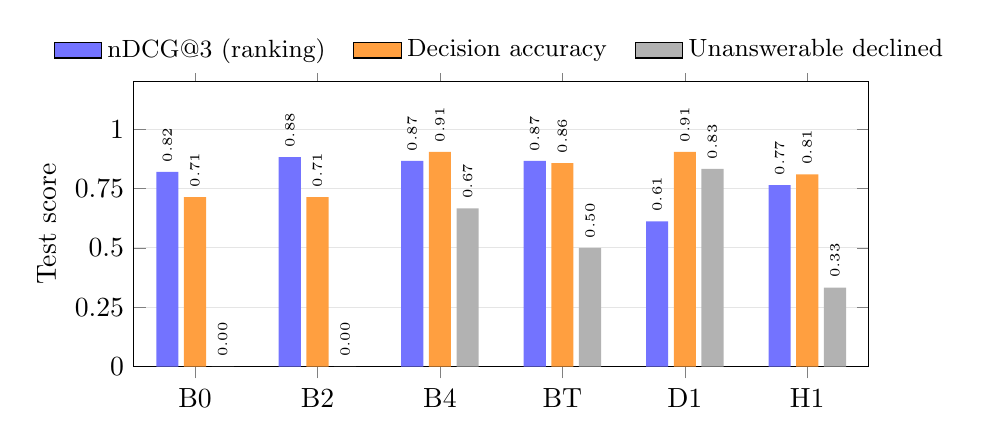
\begin{tikzpicture}
\begin{axis}[ybar, bar width=8pt, width=0.9\linewidth, height=5.2cm,
  ymin=0, ylabel={Test score},
  symbolic x coords={B0,B2,B4,BT,D1,H1}, xtick=data,
  area legend, ymax=1.2, ytick={0,0.25,0.5,0.75,1},
  legend style={at={(0.5,1.03)},anchor=south,legend columns=-1,font=\small,draw=none,/tikz/every even column/.append style={column sep=8pt}},
  nodes near coords={\pgfmathprintnumber[fixed,fixed zerofill,precision=2]{\pgfplotspointmeta}},
  every node near coord/.append style={font=\tiny, rotate=90, anchor=west},
  enlarge x limits=0.1, ymajorgrids, grid style={gray!20}]
\addplot[fill=blue!55, draw=none] coordinates {(B0,0.820) (B2,0.882) (B4,0.867) (BT,0.867) (D1,0.612) (H1,0.765)};
\addplot[fill=orange!75, draw=none] coordinates {(B0,0.714) (B2,0.714) (B4,0.905) (BT,0.857) (D1,0.905) (H1,0.810)};
\addplot[fill=gray!60, draw=none] coordinates {(B0,0.000) (B2,0.000) (B4,0.667) (BT,0.500) (D1,0.833) (H1,0.333)};
\legend{nDCG@3 (ranking), Decision accuracy, Unanswerable declined}
\end{axis}
\end{tikzpicture}
\caption{Held-out test scores for selected configurations. The threshold (B4/BT) is what lets the system decline. Dense retrieval (D1) declines well but ranks poorly and wrongly declines 1 of 15 answerable questions.}\label{fig:test-bars}
\end{figure}

\begin{takeaway}
\textbf{In plain terms.} The starter system answered \emph{every} question, including ``What will the average salary be in 2030?'', by matching words like ``this'' and ``job''. The tuned system declines half of the unanswerable test questions without turning away any answerable one, and finds a relevant ad in its top three for 14 of 15 answerable questions.
\end{takeaway}

\begin{figure}[H]\centering
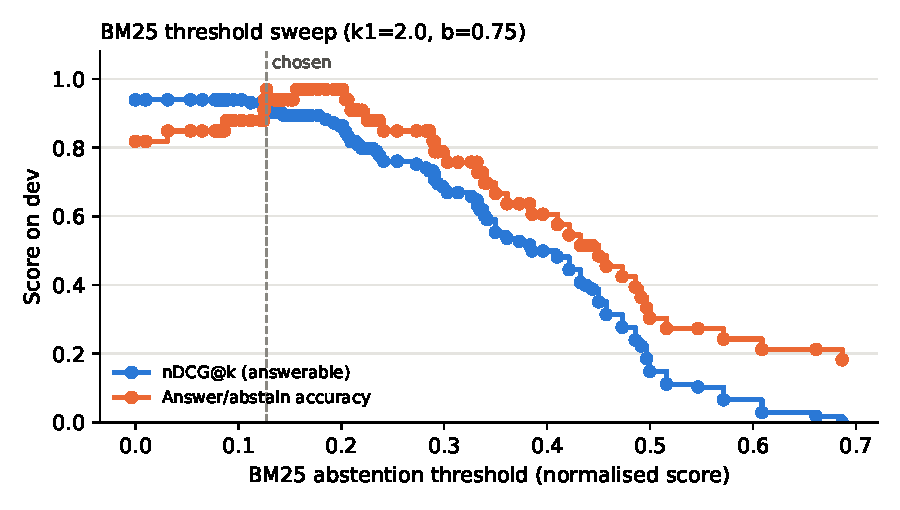
\includegraphics[width=0.78\linewidth]{img/threshold_sweep.pdf}
\caption{Effect of the decline threshold on the dev questions (k1=2.0, b=0.75). Raising it improves the answer/decline decision (orange) until it starts rejecting good evidence, after which ranking quality (blue) falls. The chosen value (0.128, dashed) sits in the middle of the best range.}\label{fig:sweep}
\end{figure}

The main results are:

\begin{enumerate}
  \item \textbf{The decline threshold is the most valuable single change.} Normalising the score and adding a threshold (B4) raised test decision accuracy from 0.714 to 0.905. Stopwords and stemming mainly helped ranking (nDCG@3 0.820 to 0.882).
  \item \textbf{The chosen system improves on the baseline, with honest uncertainty.} BT: selection score 0.862 (95\% CI 0.752--0.953), nDCG@3 0.867 (0.720--0.983), decision accuracy 0.857 (0.714--1.000). The intervals are wide because the test set has only 21 questions, and the lower bound of the selection-score interval is just below the baseline's 0.767.
  \item \textbf{A simpler step scored slightly higher on test.} B4 (0.886) beat the fully tuned BT (0.862) on test. We still report BT, because it was chosen on dev before test was seen. Swapping it after seeing test results would overstate performance.
  \item \textbf{Keyword search beat neural search on this data.} Dense MiniLM ranked worse on both dev (nDCG 0.806 vs 0.920) and test (0.612 vs 0.867). Job-ad questions hinge on exact tool names (SQL, Tableau, R), and keyword matching handles these well. The hybrid did not beat BM25 on dev. Because it answers whenever \emph{either} retriever finds evidence, it also declined fewer unanswerable questions (dev 0.50 vs 0.83).
\end{enumerate}

\paragraph{Where it fails.} The remaining errors show the limits of keyword matching. On test, ``Do I need Kubernetes certification?'' retrieved ads that mention some other \emph{certification}, and ``Will the company pay my tuition fees?'' retrieved ads that mention a \emph{university}. On dev, ``Is the R language asked for?'' matched an ad about staff speaking 70 \emph{languages}. ``Is SQL knowledge expected for business analysts?'' ranked first an ad that repeats ``knowledge'', ``expected'' and ``business analyst'' but never mentions SQL. In each case a common word in the question outweighed the missing key term.

\subsection{RQ2: grounded answers from a small local model}\label{sec:rq2}

\begin{table}[H]
\caption{End-to-end generation results with Llama 3.2 3B. Dev = the 33 dev questions (27 answerable, 6 unanswerable). Demo = 49 realistic student questions (automatic checks only).}\label{tab:gen}
\small
\begin{tabular}{lcccc}
\toprule
 & \multicolumn{2}{c}{Dev questions} & \multicolumn{2}{c}{49 demo questions} \\
\cmidrule(lr){2-3}\cmidrule(lr){4-5}
 & Prompt v2 & Prompt v3 & Prompt v2 & Prompt v3 \\
\midrule
Answerable questions answered & 27/27 & 27/27 & 40/40 & 38/40 \\
Unanswerable questions refused & 6/6 & 6/6 & 9/9 & 9/9 \\
Answers with valid citations & 22/27 (81\%) & 24/27 (89\%) & 29/40 (73\%) & 29/38 (76\%) \\
Invalid (made-up) citation IDs & 0 & 0 & 0 & 0 \\
\textbf{Faithful to sources} & \textbf{22/27 (81\%)} & \textbf{20/27 (74\%)} & -- & -- \\
\textbf{Correct answer} & \textbf{25/27 (93\%)} & \textbf{22/27 (81\%)} & -- & -- \\
Median response time & -- & -- & 7\,s & 8\,s \\
\bottomrule
\end{tabular}

\smallskip
\begin{minipage}{0.95\linewidth}\footnotesize
Faithful and correct were judged by one AI annotator (Section~\ref{sec:eval}). Demo counts include two corrections found while checking the v2 run: one answer (``Are government BA roles available?'') was wrongly logged as a refusal by the first refusal detector, which was then fixed; and ``Will this job sponsor my visa?'' was re-labelled answerable because one ad states sponsorship is not available, giving 40 answerable and 9 unanswerable questions. Response times were measured on a CPU-only laptop.
\end{minipage}
\end{table}

\begin{enumerate}
  \item \textbf{Most answers are accurate.} With prompt v2, 25 of 27 answers were correct and 22 of 27 were faithful in every claim. The typical faithfulness error is not invention but \emph{misreading}. Examples: saying an ad ``does not mention'' process mapping when it lists it; crediting one ad's duties to another; counting ``two of three'' ads that ask for Python when all three do.
  \item \textbf{Refusals were reliable, and the model never invented a source ID.} Every unanswerable question was refused end to end in both question sets. Citations, when present, always pointed to real retrieved ads.
  \item \textbf{A citation is not evidence of faithfulness.} Among v2 answers, 18 of 22 \emph{cited} answers were faithful (82\%), and 4 of 5 \emph{uncited} answers were faithful (80\%). The grounding gate therefore lets some unfaithful answers through and withholds some faithful ones. It is a format check, not a truth check (Table~\ref{tab:annot} in Appendix~\ref{app:annot}).
  \item \textbf{Prompt v3 was correctly rejected.} Showing the citation format by example (v3) raised dev citations from 22 to 24 of 27. But faithfulness fell from 22 to 20 and correctness from 25 to 22. On the demo list it also wrongly refused two answerable questions, including ``Do I need SQL to become a data analyst?''. More citations did not mean better answers, so v2 stayed in use. Prompt v4, the current default, additionally forbids placeholder counts. It has only been tried on individual questions in the app, and one of those produced an uncited draft (QA-02), so it still needs a full evaluation run.
\end{enumerate}

\subsection{RQ3: skill profiles, their accuracy, and how entry-level the evidence is}\label{sec:rq3}

Table~\ref{tab:skills} shows the deterministic skill profile per role. These counts are exactly what the skill-gap table uses. They are reproducible, and every number links to its ads.

\begin{table}[H]
\caption{Most frequently named skills per role (number of ads naming the skill / ads in the role).}\label{tab:skills}
\small
\begin{tabularx}{\linewidth}{lrY}
\toprule
Role & Ads & Top skills \\
\midrule
Data Analyst & 80 & Communication 39, SQL 38, Excel 26, Tableau 21, Data Visualisation 18, Problem Solving 15, ETL 13, Power BI 12 \\
Business/Data Analyst & 58 & Communication 39, Excel 37, Business Analysis 17, Stakeholder Management 15, SQL 14, Data Visualisation 13, Teamwork 13, Agile 12 \\
Data Scientist & 21 & Python 17, Machine Learning 13, R 13, SQL 13, Statistics 13, Communication 8, Forecasting 8, Problem Solving 7 \\
\bottomrule
\end{tabularx}
\end{table}

The profiles are distinctive and intuitive. SQL dominates technical requirements for data analysts (48\% of ads), Excel for business analysts (64\%), and Python for data scientists (81\%). Communication is the most-named skill in two of three roles. Tableau (21 ads) out-numbers Power BI (12) among data analyst ads. This reflects 2018 and should not be read as today's market.

\paragraph{The counts can be trusted, with known weak spots.} Against blind labels on 20 random ads, the tagger scored \textbf{precision 0.95, recall 0.88, F1 0.92}. Its errors are almost all soft skills. It misses wordings outside its list (``attention to details'', ``cleansing'' without ``data''), and it counts ``collaboration'' in a company's culture blurb as a Teamwork requirement. Technical skills, which drive most graduate decisions, were almost always tagged correctly. In the 72-pair label audit, \textbf{70 (97\%)} relevance labels were correct. Both errors were the same bug: two ads were tagged ``Power BI'' only because a Microsoft customer-story URL inside the ad contains \texttt{power-bi}. Soft-skill shares should therefore be read as approximate. URLs should be stripped before tagging in the next iteration.

\paragraph{Entry-level evidence is scarce.} When we checked how ``graduate'' the evidence really is, the result changed the design. Of the 159 ads, only \textbf{6} are explicit early-career candidates (4 with graduate/junior titles and no conflicting years, 2 asking for 0--1 year). 49 ask for 2+ years, and 104 do not state a requirement. Across the entire 30,000-ad file, only 9 graduate/junior ads name two or more data skills, so this source \emph{cannot} supply a graduate-only knowledge base. We therefore kept all 159 ads, added a job-level filter, and labelled filtered results as not separately validated, rather than quietly calling all ads ``graduate''.

\subsection{Key failures and what we learned}\label{sec:fail}

Several ideas did not work. Each taught us something that shaped the final system (full log in Appendix~\ref{app:log}).

\begin{description}[leftmargin=0pt]
  \item[Tuning on toy data overfits.] With 3 synthetic documents and 4 dev questions, the first threshold sat at the edge of the best range and rejected an answerable test question (test nDCG 0.0 vs 1.0 untuned). \emph{Lesson:} a small dev set cannot separate configurations. This led to the midpoint threshold rule, normalised scores, and the move to 54 real questions.
  \item[Generic questions were refused.] The app's own default question, ``What skills are requested for this role?'', was declined. After stopword removal it is ``skill request role'', words found in nearly every ad, so nothing cleared the threshold. None of the 54 evaluation questions was role-level, so tuning never saw the case. \emph{Lesson:} a test set only protects you from the failures it contains. We added a deterministic overview route instead of lowering the threshold, which would have broken refusals.
  \item[A fix that would have inflated our own scores.] Boosting ads whose skill tags contain the queried skill would fix two dev failures. We rejected it because the relevance labels come from the same tags, so the gain would be circular. \emph{Lesson:} check whether a change is evaluated by the data it was built from. The label audit (97\% correct) later confirmed the tags were good enough to use as labels, which a skill boost could not have shown.
  \item[A citation check that looked like a truth check.] We assumed that forcing citations would force faithful answers. The annotation showed otherwise: cited and uncited answers were equally faithful (82\% vs 80\%). \emph{Lesson:} an automatic check measures what it measures (here, format), not what we hope it measures. Faithfulness has to be judged against the source text.
  \item[Hybrid retrieval weakened refusal.] Merging two retrievers with OR logic means either one can force an answer. \emph{Lesson:} combining systems can combine their weaknesses. An AND-gated hybrid is the next experiment, and it needs a fresh test set.
  \item[The experience parser read ranges wrongly.] ``1--2 years'' was first classified from its lower bound, which put experienced roles into the entry-level filter. The first version counted ten ``1--2 years'' ads as near-entry evidence. After the fix and a re-audit of all 159 ads, only 6 early-career candidates remain. \emph{Lesson:} rules applied to free text need sampled manual checks, not only unit tests.
\end{description}
